
\documentclass[conference]{IEEEtran}
% Add the compsoc option for Computer Society conferences.
%
% If IEEEtran.cls has not been installed into the LaTeX system files,
% manually specify the path to it like:
% \documentclass[conference]{../sty/IEEEtran}
\usepackage{textcomp}
\usepackage{cite}
\usepackage{booktabs}
\usepackage{ctable}
\usepackage{multicol}
\usepackage{subfig}
\usepackage{float}
\usepackage{array}
\usepackage{array}
\usepackage{multirow}
\usepackage{graphicx}

\newcommand\MyBox[2]{
  \fbox{\lower0.75cm
    \vbox to 1.7cm{\vfil
      \hbox to 1.7cm{\hfil\parbox{1.4cm}{#1\\#2}\hfil}
      \vfil}%
  }%
}


%\usepackage{tikz}
%\usetikzlibrary{positioning}

% Some very useful LaTeX packages include:
% (uncomment the ones you want to load)


% *** MISC UTILITY PACKAGES ***
%
%\usepackage{ifpdf}
% Heiko Oberdiek's ifpdf.sty is very useful if you need conditional
% compilation based on whether the output is pdf or dvi.
% usage:
% \ifpdf
%   % pdf code
% \else
%   % dvi code
% \fi
% The latest version of ifpdf.sty can be obtained from:
% http://www.ctan.org/tex-archive/macros/latex/contrib/oberdiek/
% Also, note that IEEEtran.cls V1.7 and later provides a builtin
% \ifCLASSINFOpdf conditional that works the same way.
% When switching from latex to pdflatex and vice-versa, the compiler may
% have to be run twice to clear warning/error messages.












% *** GRAPHICS RELATED PACKAGES ***
%
\ifCLASSINFOpdf
  % \usepackage[pdftex]{graphicx}
  % declare the path(s) where your graphic files are
  % \graphicspath{{../pdf/}{../jpeg/}}
  % and their extensions so you won't have to specify these with
  % every instance of \includegraphics
  % \DeclareGraphicsExtensions{.pdf,.jpeg,.png}
\else
  % or other class option (dvipsone, dvipdf, if not using dvips). graphicx
  % will default to the driver specified in the system graphics.cfg if no
  % driver is specified.
  % \usepackage[dvips]{graphicx}
  % declare the path(s) where your graphic files are
  % \graphicspath{{../eps/}}
  % and their extensions so you won't have to specify these with
  % every instance of \includegraphics
  % \DeclareGraphicsExtensions{.eps}
\fi
% graphicx was written by David Carlisle and Sebastian Rahtz. It is
% required if you want graphics, photos, etc. graphicx.sty is already
% installed on most LaTeX systems. The latest version and documentation
% can be obtained at: 
% http://www.ctan.org/tex-archive/macros/latex/required/graphics/
% Another good source of documentation is "Using Imported Graphics in
% LaTeX2e" by Keith Reckdahl which can be found at:
% http://www.ctan.org/tex-archive/info/epslatex/
%
% latex, and pdflatex in dvi mode, support graphics in encapsulated
% postscript (.eps) format. pdflatex in pdf mode supports graphics
% in .pdf, .jpeg, .png and .mps (metapost) formats. Users should ensure
% that all non-photo figures use a vector format (.eps, .pdf, .mps) and
% not a bitmapped formats (.jpeg, .png). IEEE frowns on bitmapped formats
% which can result in "jaggedy"/blurry rendering of lines and letters as
% well as large increases in file sizes.
%
% You can find documentation about the pdfTeX application at:
% http://www.tug.org/applications/pdftex





% *** MATH PACKAGES ***
%
%\usepackage[cmex10]{amsmath}
% A popular package from the American Mathematical Society that provides
% many useful and powerful commands for dealing with mathematics. If using
% it, be sure to load this package with the cmex10 option to ensure that
% only type 1 fonts will utilized at all point sizes. Without this option,
% it is possible that some math symbols, particularly those within
% footnotes, will be rendered in bitmap form which will result in a
% document that can not be IEEE Xplore compliant!
%
% Also, note that the amsmath package sets \interdisplaylinepenalty to 10000
% thus preventing page breaks from occurring within multiline equations. Use:
%\interdisplaylinepenalty=2500
% after loading amsmath to restore such page breaks as IEEEtran.cls normally
% does. amsmath.sty is already installed on most LaTeX systems. The latest
% version and documentation can be obtained at:
% http://www.ctan.org/tex-archive/macros/latex/required/amslatex/math/





% *** SPECIALIZED LIST PACKAGES ***
%
%\usepackage{algorithmic}
% algorithmic.sty was written by Peter Williams and Rogerio Brito.
% This package provides an algorithmic environment fo describing algorithms.
% You can use the algorithmic environment in-text or within a figure
% environment to provide for a floating algorithm. Do NOT use the algorithm
% floating environment provided by algorithm.sty (by the same authors) or
% algorithm2e.sty (by Christophe Fiorio) as IEEE does not use dedicated
% algorithm float types and packages that provide these will not provide
% correct IEEE style captions. The latest version and documentation of
% algorithmic.sty can be obtained at:
% http://www.ctan.org/tex-archive/macros/latex/contrib/algorithms/
% There is also a support site at:
% http://algorithms.berlios.de/index.html
% Also of interest may be the (relatively newer and more customizable)
% algorithmicx.sty package by Szasz Janos:
% http://www.ctan.org/tex-archive/macros/latex/contrib/algorithmicx/




% *** ALIGNMENT PACKAGES ***
%
%\usepackage{array}
% Frank Mittelbach's and David Carlisle's array.sty patches and improves
% the standard LaTeX2e array and tabular environments to provide better
% appearance and additional user controls. As the default LaTeX2e table
% generation code is lacking to the point of almost being broken with
% respect to the quality of the end results, all users are strongly
% advised to use an enhanced (at the very least that provided by array.sty)
% set of table tools. array.sty is already installed on most systems. The
% latest version and documentation can be obtained at:
% http://www.ctan.org/tex-archive/macros/latex/required/tools/


% IEEEtran contains the IEEEeqnarray family of commands that can be used to
% generate multiline equations as well as matrices, tables, etc., of high
% quality.




% *** SUBFIGURE PACKAGES ***
%\ifCLASSOPTIONcompsoc
%  \usepackage[caption=false,font=normalsize,labelfont=sf,textfont=sf]{subfig}
%\else
%  \usepackage[caption=false,font=footnotesize]{subfig}
%\fi
% subfig.sty, written by Steven Douglas Cochran, is the modern replacement
% for subfigure.sty, the latter of which is no longer maintained and is
% incompatible with some LaTeX packages including fixltx2e. However,
% subfig.sty requires and automatically loads Axel Sommerfeldt's caption.sty
% which will override IEEEtran.cls' handling of captions and this will result
% in non-IEEE style figure/table captions. To prevent this problem, be sure
% and invoke subfig.sty's "caption=false" package option (available since
% subfig.sty version 1.3, 2005/06/28) as this is will preserve IEEEtran.cls
% handling of captions.
% Note that the Computer Society format requires a larger sans serif font
% than the serif footnote size font used in traditional IEEE formatting
% and thus the need to invoke different subfig.sty package options depending
% on whether compsoc mode has been enabled.
%
% The latest version and documentation of subfig.sty can be obtained at:
% http://www.ctan.org/tex-archive/macros/latex/contrib/subfig/




% *** FLOAT PACKAGES ***
%
%\usepackage{fixltx2e}
% fixltx2e, the successor to the earlier fix2col.sty, was written by
% Frank Mittelbach and David Carlisle. This package corrects a few problems
% in the LaTeX2e kernel, the most notable of which is that in current
% LaTeX2e releases, the ordering of single and double column floats is not
% guaranteed to be preserved. Thus, an unpatched LaTeX2e can allow a
% single column figure to be placed prior to an earlier double column
% figure. The latest version and documentation can be found at:
% http://www.ctan.org/tex-archive/macros/latex/base/


%\usepackage{stfloats}
% stfloats.sty was written by Sigitas Tolusis. This package gives LaTeX2e
% the ability to do double column floats at the bottom of the page as well
% as the top. (e.g., "\begin{figure*}[!b]" is not normally possible in
% LaTeX2e). It also provides a command:
%\fnbelowfloat
% to enable the placement of footnotes below bottom floats (the standard
% LaTeX2e kernel puts them above bottom floats). This is an invasive package
% which rewrites many portions of the LaTeX2e float routines. It may not work
% with other packages that modify the LaTeX2e float routines. The latest
% version and documentation can be obtained at:
% http://www.ctan.org/tex-archive/macros/latex/contrib/sttools/
% Do not use the stfloats baselinefloat ability as IEEE does not allow
% \baselineskip to stretch. Authors submitting work to the IEEE should note
% that IEEE rarely uses double column equations and that authors should try
% to avoid such use. Do not be tempted to use the cuted.sty or midfloat.sty
% packages (also by Sigitas Tolusis) as IEEE does not format its papers in
% such ways.
% Do not attempt to use stfloats with fixltx2e as they are incompatible.
% Instead, use Morten Hogholm'a dblfloatfix which combines the features
% of both fixltx2e and stfloats:
%
% \usepackage{dblfloatfix}
% The latest version can be found at:
% http://www.ctan.org/tex-archive/macros/latex/contrib/dblfloatfix/




% *** PDF, URL AND HYPERLINK PACKAGES ***
%
%\usepackage{url}
% url.sty was written by Donald Arseneau. It provides better support for
% handling and breaking URLs. url.sty is already installed on most LaTeX
% systems. The latest version and documentation can be obtained at:
% http://www.ctan.org/tex-archive/macros/latex/contrib/url/
% Basically, \url{my_url_here}.




% *** Do not adjust lengths that control margins, column widths, etc. ***
% *** Do not use packages that alter fonts (such as pslatex).         ***
% There should be no need to do such things with IEEEtran.cls V1.6 and later.
% (Unless specifically asked to do so by the journal or conference you plan
% to submit to, of course. )


% correct bad hyphenation here
\hyphenation{op-tical net-works semi-conduc-tor}


\begin{document}
%
% paper title
% can use linebreaks \\ within to get better formatting as desired
% Do not put math or special symbols in the title.
\title{Credit Card Fraud Prediction Using Naive Bayes and Support Vector Machines}


% author names and affiliations
% use a multiple column layout for up to three different
% affiliations
\author{\IEEEauthorblockN{Rahul Padmanabhan}
\IEEEauthorblockA{Sr. Fraud Prevention Analyst\\FIS\\
Email: rahul3@mail.usf.edu}

}


% use for special paper notices
%\IEEEspecialpapernotice{(Invited Paper)}




% make the title area
\maketitle

% As a general rule, do not put math, special symbols or citations
% in the abstract
\begin{abstract}
Credit card fraud causes millions of dollars in losses on an annual basis. In this paper I aim to build meta-models for fraud detection using the Naive Bayes approach and the Support Vector Machine (SVM) approach. Two neural network scoring parameters as used as part of our analysis. Real world data from a financial instituion is being tested with separate datasets for training and testing. The analysis on these datasets is based on training data for August 2016. The meta-models are tested on data for September 2016 to analyze model performance in the real world. As fraudulent transactions form a tiny percentage of overall transactions, accuracy rate is not the optimal indicator as the dataset is overbalanced. This paper shows how feature extraction can be used to get better results from a Naive Bayes approach and that SVM does not produce desirable results on overbalanced datasets.

\end{abstract}

% no keywords




% For peer review papers, you can put extra information on the cover
% page as needed:
% \ifCLASSOPTIONpeerreview
% \begin{center} \bfseries EDICS Category: 3-BBND \end{center}
% \fi
%
% For peerreview papers, this IEEEtran command inserts a page break and
% creates the second title. It will be ignored for other modes.
\IEEEpeerreviewmaketitle



\section{Introduction}
% no \IEEEPARstart
Credit card fraud costs the industry million of dollars in losses each year. Often, it is used to fund illegal activities and is considered as a security risk to the industry and the government. While it is a positive aspect that only a small percentage of credit card transactions are fraud, the problem that arises is detecting it and detected the fraud transaction without affecting a lot of valid transactions in the process. Declining valid transactions leads to decreased revenue, customer dissatisfaction and reputation loss for the financial institution. The industry average for fraud is around 15 basis points (bps). In this paper, I am going to build various meta-models to predict fraud on a transaction level using two approaches. One approach is the Naive Bayes method and the other is the SVM method. 

\subsection{Background}

FIS\textsuperscript{\textregistered} (Fidelity Information Services) is the worlds largest credit card processor. FIS\textsuperscript{\textregistered} is a Fortune 500 company and is also a member of Standard \& Poor’s 500\textsuperscript{\textregistered} Index. For security and privacy purposes, the datasets used contain no account numbers or identifying account specific information. For the same reason, the name of the financial institution whose data this is, is not disclosed. There are three methods of fraud identification from a system perspective:

\begin{enumerate}
\item \textbf{Switch declines} - at the server when the transaction comes in (e.g. invalid CVV code entered)
\item \textbf{Real Time declines} - Custom strategies to decline transactions
\item \textbf{Production impact} - Transactions are not declined but attempts to contact the customer are made in order to determine the nature of the transaction (Class)
\end{enumerate}


From a fraud detection standpoint, local models are present and our data includes the scores of two neural networks per transaction. A FICO\textsuperscript{\textregistered} generated score and a Visa\textsuperscript{\textregistered} generated score. Our dataset takes into account these local parameters and also uses the FICO\textsuperscript{\textregistered} score of the prior transaction on the same account (PAD Strat), which is indicated later.

\subsection{Dataset Information}

The features I have selected have been carefully chosen to give us the data we need while adequately masking the identity of the customer transacting. Our dataset does not contain customer specific information. The features have been chosen as they are common ones that customized fraud detection strategies are coded on. The description of each field is given in the table below. 

\begin{center}
\begin{tabular}{ | l | l | }
\hline
Field & Field Description \\ [0.5ex]
\hline\hline
Trn Typ & Type of Transaction \\
\hline
Dollar Strat & Transaction Amount \\
\hline
Transaction Tag & Valid/Fraud Indicator (CLASS) \\
\hline
Trn Pin Vrfy Cd & Valid/Invalid PIN\\
\hline
Trn Cvv Vrfy Cd & CVV Verification \\
\hline
Trn Pos Ent Cd & Point of Sale Entry \\
\hline
Sic Cd & Merchant Category Code \\
\hline
Mer Cnty Cd & Merchant Country Code \\
\hline
Usr Dat 4 & Compromise Association \\
\hline
Cryptogram Valid & EMV indiator for cryptogram validity \\
\hline
Diffzip3 & First 3 digit zip code mismatch\\
\hline
Travel\_Ent\_SIC & Travel and Entertainment Indicator\\
\hline
SIC1 & First digit of the SIC code \\
\hline
SIC2 & First Two digits of the SIC code \\
\hline
Metro & Metropolitan or rural location indicator \\
\hline
VAA Strat & Visa\textsuperscript{\textregistered} Score \\
\hline
Falcon Score Strat & FICO\textsuperscript{\textregistered} score \\
\hline
PAD Strat & PAD Score \\ [1ex]
\hline
\end{tabular}
\end{center}

%\hfill mds

\subsubsection{Naive Bayes Datasets}

 The data set sizes that I used in the Naive Bayes approach are as follows:
 \begin{center}
\begin{tabular}{ | l | l | l | l | }
\hline
Dataset & Valid & Fraud & Total Instances \\ [0.5ex]
\hline\hline
August (Training) & 1,239,752 & 1,311 & 1,241,063\\
\hline
September (Test) & 1,197,532 & 1,732 & 1,199,264 \\
\hline
\end{tabular}
\end{center}

\vspace{1mm}
%\hfill December 27, 2012

\subsubsection{SVM Datasets}

For the SVM approach, I have used a subset of these datasets. The minority class (Fraud) in the training set (August) has been over-sampled with replacement. The minority class has been over-sampled by 753\%. In this approach, I have only considered the transactions that have scored between 800 to 900 using the FICO\textsuperscript{\textregistered} neural network score. This was done because SVM is computationally expensive and processing over a million rows in the classifier libsvm in Weka was not possible due to hardware constraints. Another reason for doing so is that we found a larger number of fraudulent transactions within this range. The data set sizes that I have used in the SVM approach are as follows:
 \begin{center}
\begin{tabular}{ | l | l | l | l | }
\hline
Dataset & Valid & Fraud & Total Instances \\ [0.5ex]
\hline\hline
August (Training) & 5,730 & 1,587 & 5,916\\
\hline
September (Test) &  5,445 & 230 & 5,675 \\
\hline
\end{tabular}
\end{center}

%\vspace{1mm}


\subsection{Evaluation Metrics}

As credit card fraud forms only a tiny fraction of the overall transactions, the datasets used in this paper are considered to be imbalanced. An imbalanced dataset is termed as one where the number of positive instances is dwarfed by the number of negative instances. The performance of classifers on imbalanced datasets is diminished because they are designed to generalize from sample data and produce the simplest hypothesis that best fits the data, based on the principle of Occam’s razor.\cite{akbani2004} Due to this, the direct use of the measurement parameter "accuracy" may not be the most prudent approach. An example to justify this would be that if we use a dataset consisting of 1 million transactions and of this, only 1,000 transactions are fraud. If the model chooses to detect all transactions to be valid, the accuracy would be 99.9\%. Although 99.9\% accuracy may look good in theory, in the real world, the purpose of detecting fraud would be defeated. In this paper, I primarily use accuracy as a metric to check if the valid transactions are being correctly detected. Although I do not get rid of this metric altogther, the value of it is diminished in terms of the intended purpose of this paper.

In all datasets, the field ``\textit{Transaction Tag}'' is the class field. There are only two classes which are ``\textit{Valid}'' and ``\textit{Fraud}''. In our analysis, the definitions of the parameters in the confusion matrix are as follows:

%\noindent
%\renewcommand\arraystretch{1.5}
%\setlength\tabcolsep{0pt}
%\begin{tabular}{c >{\bfseries}r @{\hspace{0.7em}}c @{\hspace{0.4em}}c @{\hspace{0.7em}}l}
%  \multirow{10}{*}{\parbox{1.1cm}{\bfseries\raggedleft actual\\ value}} & 
%    & \multicolumn{2}{c}{\bfseries Prediction outcome} & \\
%  & & \bfseries p & \bfseries n & \bfseries total \\
%  & p$'$ & \MyBox{True}{Positive} & \MyBox{False}{Negative} & P$'$ \\[2.4em]
%  & n$'$ & \MyBox{False}{Positive} & \MyBox{True}{Negative} & N$'$ \\
%  & total & P & N &
%\end{tabular}


% \begin{tikzpicture}[
% box/.style={draw,rectangle,minimum size=2cm,text width=1.5cm,align=left}]
% \matrix (conmat) [row sep=.1cm,column sep=.1cm] {
% \node (tpos) [box,
%    label=left:\( \mathbf{p'} \),
%    label=above:\( \mathbf{p} \),
%    ] {True \\ positive};
% &
% \node (fneg) [box,
%    label=above:\textbf{n},
%    label=above right:\textbf{total},
%    label=right:\( \mathrm{P}' \)] {False \\ negative};
% \\
% \node (fpos) [box,
%   label=left:\( \mathbf{n'} \),
%    label=below left:\textbf{total},
%    label=below:P] {False \\ positive};
% &
% \node (tneg) [box,
%    label=right:\( \mathrm{N}' \),
%    label=below:N] {True \\ negative};
% \\
% };
% \node [left=.05cm of conmat,text width=1.5cm,align=right] {\textbf{actual \\ value}};
% \node [above=.05cm of conmat] {\textbf{prediction outcome}};
% \end{tikzpicture}

\begin{itemize}
\item \textbf{True Positive (TP)} - Fraud transactions correctly detected as fraud transactions
\item \textbf{True Negative (TN)} - Valid transactions correctly detected as valid transactions
\item \textbf{False Negative (FN)} - Fraud transactions incorrectly detected as validtransactions
\item \textbf{False Positive (FP)} - Valid Transactions incorrectly detected as fraud transactions
\end{itemize}

For our analysis, I rely on the following parameters:\\

\textbf{Recall}

\[recall = \frac{TP}{TP+FN}\]

\textbf{Precision}

\[precision = \frac{TP}{TP+FP}\]

\textbf{False Positive Rate}

\[False\ positive\ rate = \frac{FP}{TP}\]

\hfill

\section{Pre-processing Techniques Used}

For the purpose of this paper, I have evaluated the Naive Bayes classifier independently on the entirity of the data avaiable to us. This was done because the Naive Bayes classifer is not as computationally expensive as the SVM(libsvm) classifier. I have then used a subset of our data to compare the Naive Bayes classifier to SVM. 

\subsection{Datasets - Naive Bayes Internal Evaluation}

For the Naieve Bayes approach, complete August and September datasets have been used. I have used three names to refer to datasets that are used in the internal evaluation of the Naive Bayes classifier. Their names and descriptions are as follows:\\

\begin{itemize}
\item\textbf{Original} - Format of data unchanged\\

\item\textbf{Custom} - The field Dollar Strat, VAA Strat, Falcon Score Strat and PAD Strat have been grouped into ``buckets''. An example of this is suppose the transaction amount is in the range of \$1 to \$25, we categorize it as \$1-25. After grouping the four features into these buckets, I have converted the datasets nominal values to binary values in Weka by using NominaltoBinary in the pre-processing section. This process increases the number of features.\\

\item\textbf{SMOTE} - This dataset has the same number of instances and data format as the original dataset has. We have not used the ``Smoting'' technique in this dataset but it is named after it because the idea of using this approach came from reading the paper about ``SMOTE'' - Synthetic Minority Oversampling Technique\cite{chawla2002smote}. Previous work (Japkowicz, 2000) indicated that over-sampling the minority class could be one of the effective methods of dealing with an imbalanced dataset\cite{japkowicz2000learning}. In this dataset we have oversampled the minority class (Fraud) with replacement. I used fraud transactions (a total of 12,400) from January 2016 to July 2016 and added them to the dataset by randomly removing 12,400 instances of the valid class.\\

\end{itemize}

\subsection{Datasets - SVM}

The dataset that I have used in this approach is a subset of the SMOTE dataset above. I only consider the transactions that scored between 800 to 900 using the FICO\textsuperscript{\textregistered} neural network score. 10-fold cross validation is performed on the dataset for August and it is tested on the unseen data in September. To implement the \textit{libsvm} classifier we need to ensure that each data instance is represented as a vector of real numbers. We need to convert our nominal data into the numeric format. For example, a four category attribute such as \{boxing, basketball, football, chess\} would be represented as (0,0,0,1), (0,0,1,0), (0,1,0,0) and (1,0,0,0) respectively. To do this I have pre-processed the data in Weka using the Nominal to Binary approach in the \textit{Preprocess} tab. Per instructions in the documentation, I have proceeded to perform scaling on the data by normalizing the values. Scaling is done in order to reduce the bias that occurs when some of the feature values ranges are of a much higher range compared to those in smaller ranges.

\subsection{Datatsets - Comparison Between Naive Bayes and SVM}

Due to the large size of the dataset, I cannot use the datasets that I have used in the Naive Bayes approach for SVM due to the time required for computation. As a result, I have used the dataset that I have used in SVM to evaluate the Naive Bayes classifier for the purpose of comparison i.e. only the transactions that scored between 800 to 900 using the FICO\textsuperscript{\textregistered} neural network score in the \textit{SMOTE} dataset. Over sampling by replacement is maintained.


\section{Naive Bayes Classifier Approach}

The Naive Baye’s classifier is a common statistical modeling technique. It allows all the attributes, for the given instance space, to be equally important and contribute towards prediction of the class. The assumption made is that these attributes are independent of each other. Alhough this may not be the case in the real world, this technique tends to outperform more complex classifiers in certain areas of data science. This method is designed for use in supervised induction tasks, in which the performance goal is to accurately predict the class of test instances and in which the training instances include class information\cite{john1995}.The Naive Bayes classifier is based on the Bayes theorem which is:

$$ P(H \mid E) = \frac{P(E \mid H) \, P(H)}{P(E)} \\$$

H is the Hypothesis, E is the given event and P(H\textbar E) represents the probability of H conditional for the given event E.\\\\\textbf{Kernel Density Estimator} - The intuition behind using this method is that it will perform well in domains that violate the normality assumption\cite{john1995}. Using the kernel density estimate, we estimate the probability density of the classes in a non parameteric manner\cite{perez2009}. In the ``Custom'' data set for example, I have used the Nominal to Binary method in Weka to pre-process the data. However, there are other features that may not have a normal distribution. 


\subsection{Internal Comparison}

Before we proceed to the comparison of Naive Bayes vs. SVM, we will analyze the Naive Bayes classifier internally and evaluate its performance on our entire dataset. Naive Bayes classifer is not as computationally expensive as the libsvm classifier so we can evaluate the results on our main dataset with over a million instances. The Naive Bayes classifier has been run in two ways which are:\\

\begin{enumerate}
\item Default
\item With Kernel Density Estimate (KDE)\\
\end{enumerate}

This is then run on the following datasets:

\begin{enumerate}
\item Original Dataset
\item Custom Dataset
\item SMOTE Dataset
\end{enumerate}

This produces six models as a result. 10-fold cross validation is run on these datasets which have the data for August. \newline 
% \\\textbf{August dataset} - The 10-fold cross validation results are as follows:

\begin{table}[h]
\caption{August dataset 10-fold Cross Validation}
\begin{center}
\begin{tabular}{ | l | l | l | l | l | l |}
\hline
Dataset & Setting & Accuracy & Recall & Precision & FPR \\ [0.5ex]
\hline\hline
Original & Default & 97.41\% & 0.759 & 0.03 & 31.9\\
\hline
Original & KDE & 99.57\% & 0.407 & 0.106 & 8.40\\
\hline
Custom & Default & 98.00\% & 0.702 & 0.036 & 26.53\\
\hline
Custom & KDE & 99.34\% & 0.461 & 0.076 & 12.19\\
\hline
SMOTE & Default & 96.75\% & 0.82 & 0.229 & 3.36\\
\hline
SMOTE & KDE & 98.66\% & 0.675 & 0.434 & 1.30\\ [1ex]
\hline
\end{tabular}
\end{center}
\end{table}

\textit{Observations on 10-fold cross validation table}: Regarding fraud detection, the Naive Bayes - Default classifier on the SMOTE dataset detects 82\% of the overall fraud. However, if we also weigh the results of the FPR in our determination of the best performance, we could argue that the Naive Bayes - KDE classifier on the SMOTE dataset is the best performing because although the recall is 0.675 i.e. it detected 67.5\% of the overall fraud, it only misclassified 1.3 valid transactions per fraud transaction correctly classified.


\begin{table}[h]
\caption{September (Test data) Analysis}
\begin{center}
\begin{tabular}{ | l | l | l | l | l | l |}
\hline
Dataset & Setting & Accuracy & Recall & Precision & FPR \\ [0.5ex]
\hline\hline
Original & Default & 97.34\% & 0.737 & 0.039 & 24.61\\
\hline
Original & KDE & 99.51\% & 0.359 & 0.117 & 7.57\\
\hline
Custom & Default & 97.51\% & 0.725 & 0.041 & 23.33\\
\hline
Custom & KDE & 99.39\% & 0.379 & 0.096 & 9.37\\
\hline
SMOTE & Default & 96.85\% & 0.761 & 0.034 & 28.34\\
\hline
SMOTE & KDE & 98.91\% & 0.556 & 0.073 & 12.76\\ [1ex]
\hline
\end{tabular}
\end{center}
\end{table}

\begin{figure}
  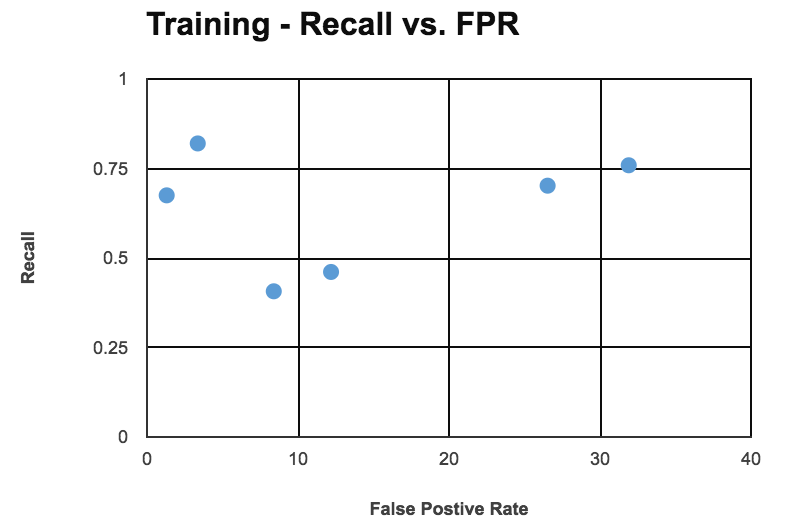
\includegraphics[width=6.7cm]{Training.png}
  \caption{Training Dataset - Recall vs FPR}
  \label{fig:testing}
\end{figure}

\begin{figure}
  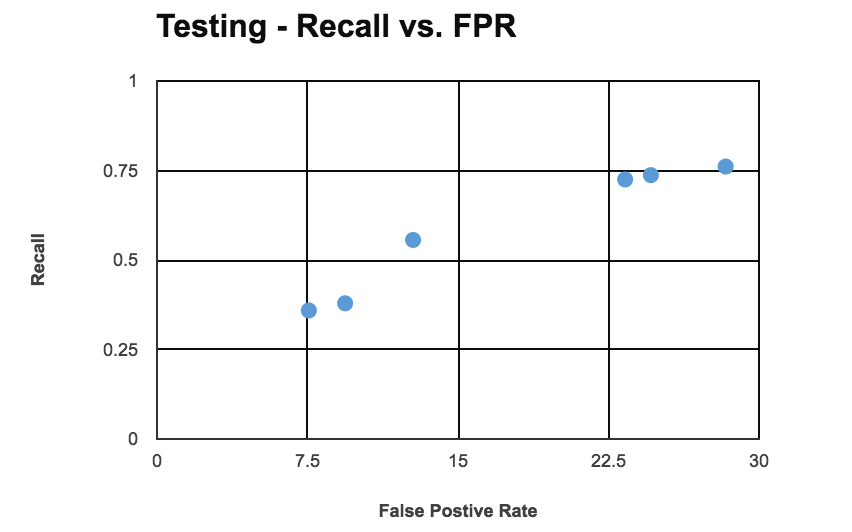
\includegraphics[width=7cm]{Testing.png}
  \caption{Test Dataset - Recall vs FPR}
  \label{fig:testing}
\end{figure}


\newpage
\textit{Observations}: If we were to set a threshold stating that at least 50\% of the overall fraud needs to be detected and the FPR below 15 then the Naive Bayes - KDE on the SMOTE dataset would win. It seems to be the most feasible option once we take the valid impact i.e. FPR into consideration. Although the same combination had an FPR of 1.3 on the training set, it has performed far worse on the test set with a decrease in recall and an increase in FPR. In the graphs above, the optimal space is the top left quadrant. We see that while the 10-fold cross validation does well in that regard, the graph on the unseen data does not.

\section{Support Vector Machine Approach}

In classification problems, linear models can be very effective and simple.  But in real world scenarios, data is seldom linearly separable. Linear classifiers (as the name suggests) fail to classify non-linear boundaries. The limitation of linear models can be addressed by using Support Vector Machines (SVM). SVM is less susceptible to overfitting because of a learned decision boundary called the \textit{maximum margin hyperplane}. It uses a \textit{kernel trick} to do the non-linear mapping. SVM only considers data points close to the hyperplane, treats the instances as \textit{support vectors} and ignores the rest. The data is projected from the original space to a higher dimension space. This allows non-linear boundaries on the data in the original space. 


Previous work has identified that support vector machines tend to perform badly on imbalanced datasets\cite{akbani2004}. In this paper, for SVM purposes, we use the SMOTE dataset with FICO\textsuperscript{\textregistered} scores ranging between 800 to 900 to analyze the overall performance. We have used the libsvm classifier in Weka that was downloaded as separate plugin. In order to gauge which settings are optimal for \textit{libsvm} we have using the \textit{C-Support Vector Classification} (SVM-C) with the following kernels:

\begin{enumerate} 
\item Linear
\item Radial Basis Function (RBF)
\item Polynomial
 \end{enumerate}

A manual coarse grid search has been done to evaluate the model for the optimal values of ${\gamma}$ and \textit{C}.
${\gamma}$ is a parameter of the Gaussian Radial Basis function and \textit{C} is the cost of error. High values of ${\gamma}$ are known to produce low variance models and with a high bias and low values of ${\gamma}$ produce the opposite. We have done a 10-fold cross validation with the values of gamma and \textit{C} using a coarse grid search\cite{chang2011libsvm}. Due to time constraints, the fine grid search is placed outside the scope of this paper. As this dataset is imbalanced, we assume that high values of \textit{C} will yield us a low minimum margin separating hyperplane.\\

Coarse Grid Search on the following:\\\\
${\gamma}$ = 2\textsuperscript{-5}, 2\textsuperscript{-4}, 2\textsuperscript{-3}, 2\textsuperscript{3}, 2\textsuperscript{4}, 2\textsuperscript{5}\\
C = 2\textsuperscript{-15}, 2\textsuperscript{-14}, 2\textsuperscript{-13}, 2\textsuperscript{13}, 2\textsuperscript{14}, 2\textsuperscript{15}
 
\begin{table}[h]
\caption{Linear Kernel - 10-fold Cross Validation}
\begin{center}
\begin{tabular}{ | l | l | l | l | l | l |}
\hline
Gamma & C & Accuracy & Recall & Precision & FPR \\
\hline\hline
2\textsuperscript{-5} & 2\textsuperscript{-15} & 73.17\% & 0 & 0 & 0 \\
\hline
2\textsuperscript{-4} & 2\textsuperscript{-14} & 73.71\% & 0 & 0 & 0 \\
\hline
2\textsuperscript{-3} & 2\textsuperscript{-13} & 73.71\% & 0 & 0 & 0 \\
\hline
2\textsuperscript{3} & 2\textsuperscript{13} & 76.35\% & 0.383 & 0.591 & 0.69 \\
\hline
2\textsuperscript{4} & 2\textsuperscript{14} & 75.7\% & 0.297 & 0.594 & 0.68 \\
\hline
2\textsuperscript{5} & 2\textsuperscript{15} & 76.98\% & 0.271 & 0.677 & 0.48 \\
\hline
\end{tabular}
\end{center}
\end{table}
 

 \begin{table}[h]
\caption{Linear kernel - Test Data Results}
\begin{center}
\begin{tabular}{ | l | l | l | l | l | l |}
\hline
Gamma & C & Accuracy & Recall & Precision & FPR \\
\hline\hline
2\textsuperscript{-5} & 2\textsuperscript{-15} & 95.94\% & 0 & 0 & 0 \\
\hline
2\textsuperscript{-4} & 2\textsuperscript{-14} & 95.94\% & 0 & 0 & 0 \\
\hline
2\textsuperscript{-3} & 2\textsuperscript{-13} & 95.94\% & 0 & 0 & 0 \\
\hline
2\textsuperscript{3} & 2\textsuperscript{13} & 17.69\% & 0.943 & 0.045 & 0.05 \\
\hline
2\textsuperscript{4} & 2\textsuperscript{14} & 95.11\% & 0.03 & 0.115 & 7.71 \\
\hline
2\textsuperscript{5} & 2\textsuperscript{15} & 94.98\% & 0.035 & 0.113 & 7.88 \\
\hline
\end{tabular}
\end{center}
\end{table}



\begin{table}[!h]
\caption{RBF kernel - 10-fold Cross Validation}
\begin{center}
\begin{tabular}{ | l | l | l | l | l | l |}
\hline
Gamma & C & Accuracy & Recall & Precision & FPR \\
\hline\hline
2\textsuperscript{-5} & 2\textsuperscript{-15} & 73.17\% & 0 & 0 & 0 \\
\hline
2\textsuperscript{-4} & 2\textsuperscript{-14} & 73.17\% & 0 & 0 & 0 \\
\hline
2\textsuperscript{-3} & 2\textsuperscript{-13} & 73.17\% & 0 & 0 & 0 \\
\hline
2\textsuperscript{3} & 2\textsuperscript{13} & 72.07\% & 0.430 & 0.477 & 1.10 \\
\hline
2\textsuperscript{4} & 2\textsuperscript{14} & 71.63\% & 0.382 & 0.465 & 1.15 \\
\hline
2\textsuperscript{5} & 2\textsuperscript{15} & 72.48\% & 0.334 & 0.481 & 1.08 \\
\hline
\end{tabular}
\end{center}
\end{table}


 \begin{table}[!h]
\caption{RBF kernel - Test Data Results}
\begin{center}
\begin{tabular}{ | l | l | l | l | l | l |}
\hline
Gamma & C & Accuracy & Recall & Precision & FPR \\
\hline\hline
2\textsuperscript{-5} & 2\textsuperscript{-15} & 95.94\% & 0 & 0 & 0 \\
\hline
2\textsuperscript{-4} & 2\textsuperscript{-14} & 95.94\% & 0 & 0 & 0 \\
\hline
2\textsuperscript{-3} & 2\textsuperscript{-13} & 95.94\% & 0 & 0 & 0 \\
\hline
2\textsuperscript{3} & 2\textsuperscript{13} & 93.42\% & 0.026 & 0.039 & 0.04 \\
\hline
2\textsuperscript{4} & 2\textsuperscript{14} & 93.85\% & 0.030 & 0.053 & 18.00 \\
\hline
2\textsuperscript{5} & 2\textsuperscript{15} & 94.07\% & 0.013 & 0.027 & 0.03 \\
\hline
\end{tabular}
\end{center}
\end{table}


\begin{table}[!h]
\caption{Polynomial kernel - 10-fold Cross Validation}
\begin{center}
\begin{tabular}{ | l | l | l | l | l | l |}
\hline
Gamma & C & Accuracy & Recall & Precision & FPR \\
\hline\hline
2\textsuperscript{-5} & 2\textsuperscript{-15} & 73.17\% & 0 & 0 & 0 \\
\hline
2\textsuperscript{-4} & 2\textsuperscript{-14} & 73.17\% & 0 & 0 & 0 \\
\hline
2\textsuperscript{-3} & 2\textsuperscript{-13} & 73.17\% & 0 & 0 & 0 \\
\hline
2\textsuperscript{3} & 2\textsuperscript{13} & 62.12\% & 0.498 & 0.354 & 1.83 \\
\hline
2\textsuperscript{4} & 2\textsuperscript{14} & 60.9\% & 0.491 & 0.341 & 1.93 \\
\hline
2\textsuperscript{5} & 2\textsuperscript{15} & 60.15\% & 0.471 & 0.330 & 2.03 \\
\hline
\end{tabular}
\end{center}
\end{table}


 \begin{table}[!h]
\caption{Polynomial kernel - Test Data Results}
\begin{center}
\begin{tabular}{ | l | l | l | l | l | l |}
\hline
Gamma & C & Accuracy & Recall & Precision & FPR \\
\hline\hline
2\textsuperscript{-5} & 2\textsuperscript{-15} & 18.73\% & 0.900 & 0.043 & 22.17 \\
\hline
2\textsuperscript{-4} & 2\textsuperscript{-14} & 22.78\% & 0.887 & 0.977 & 21.35 \\
\hline
2\textsuperscript{-3} & 2\textsuperscript{-13} & 30.48\% & 0.800 & 0.045 & 21.19 \\
\hline
2\textsuperscript{3} & 2\textsuperscript{13} & 14.76\% & 0.952 & 0.043 & 22.04 \\
\hline
2\textsuperscript{4} & 2\textsuperscript{14} & 12.26\% & 0.961 & 0.043 & 22.49 \\
\hline
2\textsuperscript{5} & 2\textsuperscript{15} & 11.52\% & 0.965 & 0.042 & 22.58 \\
\hline
\end{tabular}
\end{center}
\end{table}
 
\break
From this, we observe that the SVM does not have the best performance when it comes to classifying a valid transaction correctly. We notice that when the recall increases, the accuracy decreased beyond an acceptable threshold. SVM performs well on the training set in 10-fold cross validation however, the performance is worse on the test data. Of the three kernels evaluated, the polynomial kernel gives us the best results in terms of recall. However, it runs at a low accuracy rate and high FPR. We also need to keep in mind that using the polynomial kernel is computationally expensive.
 
\section{Comparison of Naïve Bayes vs SVM}
 
Previously, in the Naive Bayes analysis, I have considered the entire dataset for August and September which was over a million instances in each case. To accurately compare this approach to SVM we will be using the same dataset that was used for SVM, the SMOTE dataset with FICO\textsuperscript{\textregistered} scores from 800-900. We will then analyze the performance of Naïve Bayes with and without the kernel density estimator on this dataset. The results are as follows:


 \begin{table}[!h]
\caption{Naive Bayes On The Same Training Data as SVM - 10-Fold Cross Validation}
\begin{center}
\begin{tabular}{ | l | l | l | l | l |}
\hline
Type & Accuracy & Recall & Precision & FPR \\
\hline\hline
Default & 92.59\% & 0.21 & 0.118 & 7.462 \\
\hline
KDE & 96.29\% & 0.048 & 0.176 & 4.667 \\
\hline
\end{tabular}
\end{center}
\end{table}


 \begin{table}[!h]
\caption{Naive Bayes On The Same Test Data as SVM}
\begin{center}
\begin{tabular}{ | l | l | l | l | l |}
\hline
Type & Accuracy & Recall & Precision & FPR \\
\hline\hline
Default & 90.41\% & 0.117 & 0.073 & 12.63 \\
\hline
KDE & 95.4\% & 0.004 & 0.030 & 32 \\
\hline
\end{tabular}
\end{center}
\end{table}



% An example of a floating figure using the graphicx package.
% Note that \label must occur AFTER (or within) \caption.
% For figures, \caption should occur after the \includegraphics.
% Note that IEEEtran v1.7 and later has special internal code that
% is designed to preserve the operation of \label within \caption
% even when the captionsoff option is in effect. However, because
% of issues like this, it may be the safest practice to put all your
% \label just after \caption rather than within \caption{}.

% Reminder: the "draftcls" or "draftclsnofoot", not "draft", class
% option should be used if it is desired that the figures are to be
% displayed while in draft mode.

% \begin{figure}[!t]
% \centering
% \includegraphics[width=2.5in]{myfigure}
% where an .eps filename suffix will be assumed under latex, 
% and a .pdf suffix will be assumed for pdflatex; or what has been declared
% via \DeclareGraphicsExtensions.
% \caption{Simulation Results.}
% \label{fig_sim}
% \end{figure}

% Note that IEEE typically puts floats only at the top, even when this
% results in a large percentage of a column being occupied by floats.


% An example of a double column floating figure using two subfigures.
% (The subfig.sty package must be loaded for this to work.)
% The subfigure \label commands are set within each subfloat command,
% and the \label for the overall figure must come after \caption.
% \hfil is used as a separator to get equal spacing.
% Watch out that the combined width of all the subfigures on a 
% line do not exceed the text width or a line break will occur.

% \begin{figure*}[!t]
% \centering
% \subfloat[Case I]{\includegraphics[width=2.5in]{box}%
% \label{fig_first_case}}
% \hfil
% \subfloat[Case II]{\includegraphics[width=2.5in]{box}%
% \label{fig_second_case}}
% \caption{Simulation results.}
% \label{fig_sim}
% \end{figure*}

% Note that often IEEE papers with subfigures do not employ subfigure
% captions (using the optional argument to \subfloat[]), but instead will
% reference/describe all of them (a), (b), etc., within the main caption.


% An example of a floating table. Note that, for IEEE style tables, the 
% \caption command should come BEFORE the table. Table text will default to
% \footnotesize as IEEE normally uses this smaller font for tables.
% The \label must come after \caption as always.
%
%\begin{table}[!t]
%% increase table row spacing, adjust to taste
%\renewcommand{\arraystretch}{1.3}
% if using array.sty, it might be a good idea to tweak the value of
% \extrarowheight as needed to properly center the text within the cells
%\caption{An Example of a Table}
%\label{table_example}
%\centering
%% Some packages, such as MDW tools, offer better commands for making tables
%% than the plain LaTeX2e tabular which is used here.
%\begin{tabular}{|c||c|}
%\hline
%One & Two\\
%\hline
%Three & Four\\
%\hline
%\end{tabular}
%\end{table}


% Note that IEEE does not put floats in the very first column - or typically
% anywhere on the first page for that matter. Also, in-text middle ("here")
% positioning is not used. Most IEEE journals/conferences use top floats
% exclusively. Note that, LaTeX2e, unlike IEEE journals/conferences, places
% footnotes above bottom floats. This can be corrected via the \fnbelowfloat
% command of the stfloats package.

\subsection{Success Determination}

In August, 43\% of the overall fraud was declined by existing fraud strategies and the number reduced to 36\% in September.  This number excludes the \textit{switch declines} that we spoke of earlier.  Our focus was on keeping the false positive ratio below 3 and improving the detection percentage to 25\% over the existing declined percentage.

\section{Conclusion}

In the internal analysis of Naive Bayes, I can conclude that the default (without KDE) has lower accuracy and higher FPR but has higher recall on both the training and testing datasets. The Naive Bayes with KDE has higher accuracy and lower FPR but has a lower recall on both the training and testing datasets.

From the analysis done for the evaluation of Naive Bayes vs. SVM, I can conclude that while both the approaches perform poorly in terms of anomaly detection, the SVM approach performed better than Naive Bayes on the test data set with 10-fold cross validation. The Polynomial kernel with ${\gamma}$ of 2\textsuperscript{3} and \textit{C} of 2\textsuperscript{13} detects 49.8\% of the overall fraud.

In terms of unseen test data, the SVM approach with RBF Kernel having ${\gamma}$ of 2\textsuperscript{3} and \textit{C} of 2\textsuperscript{13} is the most feasible option has it has a recall of 0.026, FPR of 0.04 and accuracy of 93.42\%.

From a different standpoint, if we evaluate all the classifiers using only \textit{recall}, the SVM with the polynomial kernel outperforms Naive Bayes as it reaches a maximum recall of 0.965 for the values that we tested i.e. with a ${\gamma}$ of 2\textsuperscript{5} and \textit{C} of 2\textsuperscript{15}. The catch to this is that the FPR is 22.58 and accuracy of only 11.52\% which in the real world would decline an unacceptable number of valid transactions.



\section{Future Work}
For future work, I would like to evaluate other classifiers such as decision trees and evaluate the performance on credit card fraud detection. Due to system hardware limitations, I was not able to evaluate the entire dataset on the \textit{libsvm} classifier. In the future I would like to run a larger sample of the data against the SVM classifier to analyze its performance. In this paper, although I have called the dataset the \textit{SMOTE} dataset, it was done by over sampling of the minority class with replacement. This causes us to lose good examples of the majority class and we fail to utilize those instances for training as a result. I would like to generate synthetic examples without under sampling the majority class in the future. In this paper, I have not evaluated the sigmoid kernel in the \textit{libsvm} classifier. This is another path to explore in the future.

% conference papers do not normally have an appendix


% use section* for acknowledgement






% trigger a \newpage just before the given reference
% number - used to balance the columns on the last page
% adjust value as needed - may need to be readjusted if
% the document is modified later
%\IEEEtriggeratref{8}
% The "triggered" command can be changed if desired:
%\IEEEtriggercmd{\enlargethispage{-5in}}

% references section

% can use a bibliography generated by BibTeX as a .bbl file
% BibTeX documentation can be easily obtained at:
% http://www.ctan.org/tex-archive/biblio/bibtex/contrib/doc/
% The IEEEtran BibTeX style support page is at:
% http://www.michaelshell.org/tex/ieeetran/bibtex/
%\bibliographystyle{IEEEtran}
% argument is your BibTeX string definitions and bibliography database(s)
%\bibliography{IEEEabrv,../bib/paper}
%
% <OR> manually copy in the resultant .bbl file
% set second argument of \begin to the number of references
% (used to reserve space for the reference number labels box)
% \nocite(*)
\bibliographystyle{IEEEtran}
\bibliography{ref}


%\bibitem{IEEEhowto:kopka}
%H.~Kopka and P.~W. Daly, \emph{A Guide to \LaTeX}, 3rd~ed.\hskip 1em plus
%  0.5em minus 0.4em\relax Harlow, England: Addison-Wesley, 1999.






% that's all folks
\end{document}


